% vim: tw=80

\chapter{Introduction}

The field of particle physics is driven by the desire to provide answers to the
questions about the fundamental constituents of matter and the interactions
between them. The collision of particles at high energies and the analysis of
their scattering byproducts is an excellent method to gain deep insights into
the fundamental principles of our universe.

In the endeavor to reach highest energies in order to produce very rare particles and
search for new physics, particle accelerators became ever bigger and more
complex. Today's most powerful collider is the Large Hadron Collider (LHC).

In the LHC, protons are accelerated to unprecedented energies and brought to
collision. The constituents of the protons, quarks and gluons, interact and can
produce a plethora of particles. Their decay products are detected and
measured precisely in huge particle detectors installed at the LHC, such as the
Compact Muon Solenoid (CMS) detector.

Quarks and gluons which are produced in the collision manifest themselves as
streams of collimated particles in the detector and are clustered into so-called
jets. The measurement of events containing two such jets with large
transverse momenta, dijet events, allow for rigorous tests of predictions of
Quantum Chromodynamics (QCD). The jets can be measured precisely in the CMS
detector and theory predictions exist at next-to-leading order accuracy.
Ultimately, the knowledge of the proton structure can be improved by comparing
measurement and theory prediction and deriving constraints.

The structure of the proton is described by parton distribution functions (PDFs) which
give the probability to find a quark or gluon at a energy scale $Q$ with a fractional
momentum $x$ of the proton. The $x$ dependence is not predicted by QCD but has
to be parametrized and determined from fits to experimental data.

In this thesis, a measurement of triple-differential dijet cross sections at the
LHC is explored for the first time. The cross section is measured as a function
of the average transverse momentum of the dijets, \ptavg, the rapidity
separation \ystar and the boost of the dijet system, \yboost. The
triple-differential measurement allows to separate phase space regions that are
sensitive sensitive to the PDFs and those that are not.
Fig.~\ref{fig:intro_ybys_hint} illustrates the various dijet event topologies
that can be measured in this analysis. Especially the boosted region offers a
high sensitivity as the probed $x$ of both protons must be very different to
boost both jets to the same side. Consequently, $x_1$ or $x_2$ must be very
large in order to reach high transverse momenta. However, the PDFs are not very
well known in the high-$x$ region. Thus, contraints on the PDFs can be extracted
if the measurement is sufficiently precise.

\begin{SCfigure}[][h!tp]
    \centering
    \caption[Illustration of dijet topologies various \ystar and \yboost bins]{
             Illustration of dijet event topologies which can be measured in
             the various \ystar and \yboost bins. Especially the boosted region
             is very sensitive to the PDFs. To boost both jets to the same side,
             very different $x$ of the incoming protons must be probed. To reach
             large transverse momentum, $x_1$ or $x_2$ must be very high.}
    \label{fig:intro_ybys_hint}
    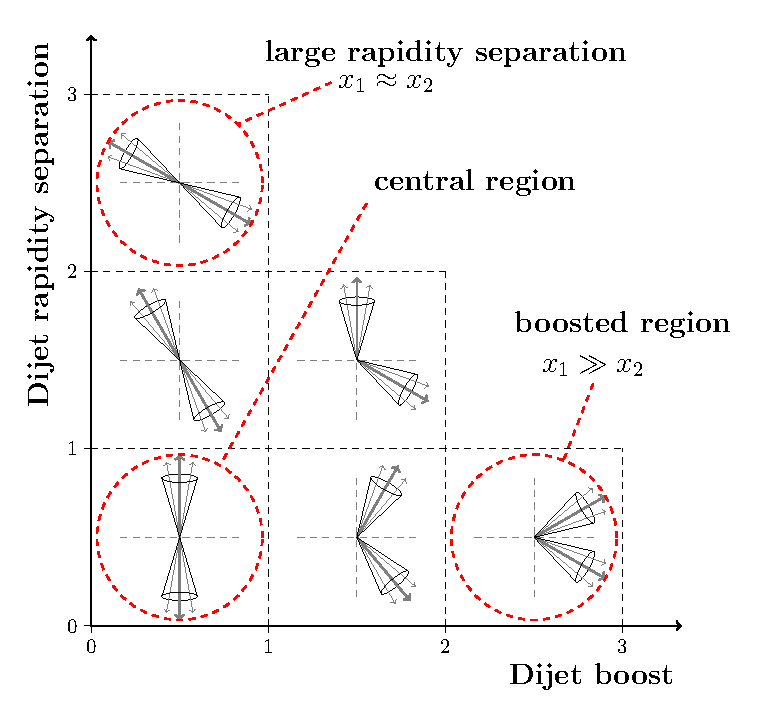
\includegraphics[width=0.5\textwidth]{figures/drawings/ybys_hint.pdf}
\end{SCfigure}

The thesis is structured as follows: In
Chapter~\ref{sec:theoretical_foundations}, the theoretical foundations for dijet
production at hadron colliders are outlined. An overview of the Standard Model
of particle physics with focus on perturbative QCD is given.  Furthermore, the
relativistic kinematics of dijet production is explained.
Chapter~\ref{sec:experimental_setup} summarizes the experimental setup of the
CMS detector and the measurement and reconstruction of jets. 

The theoretical considerations for the definition of the observables as well as
the accuracy of the NLO calculations are discussed in
Chapter~\ref{sec:theory_predictions}. The measurement of the triple-differential
dijet cross section with the CMS detector is presented in
Chapter~\ref{sec:measurement}. A multitude of studies of detector and
reconstruction efficiencies as well as the careful determination of all
uncertainties prove the reliability of the analysis.  Finally, the cross
sections are corrected for detector effects in an iterative unfolding procedure
and are compared to pQCD calculations at NLO accuracy.

The thesis is rounded off with studies of the PDFs in
Chapter~\ref{sec:pdf_constraints}. Constraints on the proton PDFs are presented.
Furthermore, a simultaneous fit of the PDFs and the strong coupling is performed
to determine the coupling most accurately.

